
\documentclass{article}

% Language setting
% Replace `english' with, e.g., `spanish' to change the document language
\usepackage[english]{babel}

% Set page size and margins
% Replace `letterpaper' with `a4paper' for UK/EU standard size
\usepackage[letterpaper,top=2cm,bottom=2cm,left=3cm,right=3cm,marginparwidth=1.75cm]{geometry}

% Useful packages

\usepackage{amsmath}
\usepackage{graphicx}
\usepackage{relsize}
\usepackage{pgfplots}
\pgfplotsset{compat=1.17}
\usepackage[colorlinks=true, allcolors=blue]{hyperref}
\usepackage{tikz}

\usetikzlibrary{shapes,arrows,positioning}
\usepackage{float} % Include the float package in your preamble

\title{Probabilistic Road Map Planning and Pure Pursuit Algorithm for Autonomous Vehicle Navigation}
\author{HAzMAT (Team 12)}

\begin{document}
\maketitle



\section{Introduction: Alonso}

For an autonomous robot to properly function, it must be able to reliably plot a course through an environment (optimized for some constraint) and execute it. Within the framework of RSS, path planning sits at the robot architecture framework's spatial perception and motion planning level. The robot must create a geometric world model to navigate between two points successfully. This lab builds upon previous labs as the particle filter used to localize the robot in Lab 5 is used to determine the start point of the robot, upon which the path planning algorithms are applied. Looking ahead to the Final Challenge, this lab is a crucial component of autonomous navigation through a city.

Autonomous vehicle navigation consists of two processes running in series: path planning and execution. Given a known environment, a robot should be able to navigate safely between any two points. The first step is planning the motion, which can take the form of a search-based or sampling-based algorithm. The implementation used in this report was sampling-based, and the relative merits of the two approaches will be discussed further in the Technical Approach section. The idea behind a sampling-based approach is to randomly sample the map space, keeping all samples corresponding to a valid pose (i.e., do not conflict with an obstacle). Those samples (nodes) are connected via edges. The combination of nodes and edges creates a graph that a search algorithm (informed or uninformed) can navigate to find an optimal path from start to end. This path, represented as a set of (x,y) coordinates, is then fed into our path executor. A pure pursuit controller is implemented to execute the desired path. On a wheeled robot, pure pursuit takes in a path (or series of points) and, using a specified look-ahead distance, adjusts the steering angle in order to intersect with the given point. With proper implementation, the autonomous robot should be able to drive safely between any two points both in simulation and in real life.



\section{Technical Approach}

\subsection{Path Planning: Alonso, Heath}

Path planning is a well-documented problem within the field of robotics. It is is essential for a robot to execute its purpose for many applications, particularly autonomous vehicle navigation. Path planning is complex to effectively solve due to the high computation expense incurred in large, multidimensional environments, particularly as many applications require high fidelity. Path planning involves the creation of a graph (made of nodes and edges), and the computation complexity scales with $O(n^2)$. 

Path planning algorithms fit into two classes: search-based and sample-based. Searched-based algorithms include the class of algorithms spanning BFS, DFS, Dijkstra, and A*. These search methods require the discretization of the configuration space, which often has to be quite fine in order to prevent collisions. While discretization is a very expensive process, search-based algorithms can guarantee resolution completeness, meaning the optimal solution is returned if a solution exists. Sampling-based methods, which include Probabilistic Road Map (PRM) and Rapidly-exploring Random Trees (RRS), on the other hand, avoid the expensive discretization by randomly sampling points on the map (keeping only those that are valid) and then create a less complex graph. In short, sample-based methods produce a less optimal path but return more quickly. The implementation used in this Lab, specifically Probabilistic Road Map, was sample-based as given the size of the map and high resolution required (due to a low margin of error for crashes), a sample-based approach seemed more appropriate. This was further strengthened by the fact that the environment remains unchanged, and no "narrow passages" cause PRM to struggle. In our sample-based implementation, PRM was selected over RRT because PRM has more parameters we could iterate upon in our implementation such as the number of randomly sampled points and the threshold distance for considering two nodes neighbors. PRM also has many advantages, such as probabilistic completeness, i.e., as the number of samples increases, the probability of finding a solution approaches unity. Furthermore, since all the data is pre-processed, it can support multiple queries, although the searches can only run after the map is constructed.

The first step in our PRM implementation is to pre-process the map. Due to the smoothing nature of pure pursuit, the robot is unlikely to follow the plotted course perfectly, and particularly around corners, there is a risk of hitting a wall. To combat this, a dilation of 10 pixels was preformed, effectively widening the obstacles (walls) in the map by altering the OccupanyGrid passed in. 10 pixels was chosen as it gives an adequate margin of safety. Each pixel unit is $\sim$5cm when converted into the map space. Therefore, a dilation with a radius of 10 pixels provides a cushion of $50\sqrt{2}$ or $\sim$70cm from any obstacle. Given that in the calculation of valid edges, the edges are discretized into 10 segments (at most 50cm on account of a neighbor distance of 5m), it would be impossible for the created graph to hit a wall, and in fact, the pre-processing supports a healthy margin of safety.

With a new, more conservative OccupancyGrid, the next step is to initialize the PRM. Through testing it became apparent that in order to achieve sufficient coverage of the map, at least 5,000 points were needed. Points are uniformly sampled in the pixel frame to obtain maximum coverage as seen in the figure below:

\begin{figure}[htbp]
  \centering
  \includegraphics[width=0.5\textwidth]{lab6_points.png}
  \caption{PRM Random Sample (2,000 Samples)}
  \label{fig:example_png}
\end{figure}


If those sampled pixels correspond to a free pixel on the map, they are kept as nodes, otherwise, they are discarded. After all the valid points are determined, edges are built between the points. There are two requirements in order to build an edge. First, the two points must be within a certain distance of each other, which we call the neighbor threshold.The neighbor threshold has to stay in balance with the number of points as with a higher number of sampled points, a lower neighbor threshold distance helps reduces computation complexity (and potentially increases the smoothness of the graph). If two points are considered neighbors, then an edge in constructed between the two points with the caveat that the edge does not intersect an occupied pixel on the Occupancy Grid. 



With the graph built, once start and end points are selected, an A* algorithm is run to connect the start and endpoints optimizing for minimum distance. The heuristic used in the A* algorithm was simple euclidean distance. Interestingly, from a lap time perspective, the shortest path is not necessarily optimal, however altering the heuristic to account for a proper racing line is outside the scope of the class. The end result is that the robot is able to plan a path from its current pose (specified in RVIZ or using a particle filter in real life) to a selected end point. The figure below shows a simplified version of an A* search.

\begin{figure}[H]
  \centering
  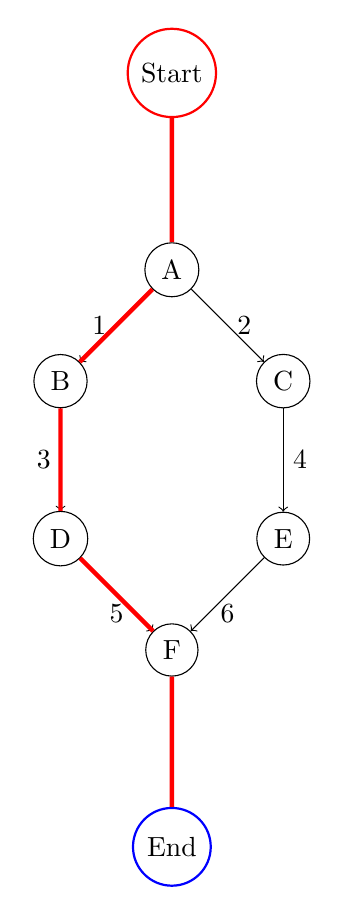
\begin{tikzpicture}[node distance=2cm, auto]
    % Nodes
    \node[circle, draw] (A) {A};
    \node[circle, draw, below left of=A] (B) {B};
    \node[circle, draw, below right of=A] (C) {C};
    \node[circle, draw, below of=B] (D) {D};
    \node[circle, draw, below of=C] (E) {E};
    \node[circle, draw, below right of=D] (F) {F};
    
    % Edges
    \draw[->] (A) -- node[midway, left] {1} (B);
    \draw[->] (A) -- node[midway, right] {2} (C);
    \draw[->] (B) -- node[midway, left] {3} (D);
    \draw[->] (C) -- node[midway, right] {4} (E);
    \draw[->] (D) -- node[midway, below] {5} (F);
    \draw[->] (E) -- node[midway, below] {6} (F);
    
    % Start and end nodes
    \node[draw=red, circle, thick, above of=A, yshift=0.5cm] (start) {Start};
    \node[draw=blue, circle, thick, below of=F, yshift=-0.5cm] (end) {End};
    
    % Path between start and end
    \draw[ultra thick, red] (start) -- (A) -- (B) -- (D) -- (F) -- (end);
  \end{tikzpicture}
  \caption{A* Algorithm}
  \label{fig:example_graph_start_end}
\end{figure}

\vspace{1cm}
The figure below summarizes the steps involved in path planning. 
\vspace{1cm}

\vspace{1cm}
\begin{figure}[htbp]
  \centering
  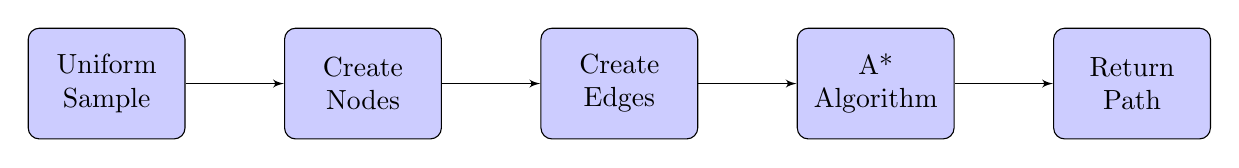
\begin{tikzpicture}[node distance=1.0cm, auto]
    % Define block styles
    \tikzstyle{block} = [rectangle, draw, fill=blue!20, text width=5.0em, text centered, rounded corners, minimum height=4.0em]
    \tikzstyle{line} = [draw, -latex']

    % Nodes
    \node [block] (Uniform_Sample) {Uniform Sample};
    \node [block, right=1.25cm of Uniform_Sample] (Create_Nodes) {Create Nodes};
    \node [block, right=1.25cm of Create_Nodes] (Create_Edges) {Create Edges};
    \node [block, right=1.25cm of Create_Edges] (A_Star_Algorithm) {A* Algorithm};
    \node [block, right=1.25cm of A_Star_Algorithm] (Return_Path) {Return Path};  

    % Arrows
    \path [line] (Uniform_Sample.east) -- (Create_Nodes.west);
    \path [line] (Create_Nodes.east) -- (Create_Edges.west);
    \path [line] (Create_Edges.east) -- (A_Star_Algorithm.west);
    \path [line] (A_Star_Algorithm.east) -- (Return_Path.west);  

  \end{tikzpicture}
  \caption{Flowchart illustrating Path Planning}
  \label{fig:scaled_flowchart_sensor_model}
\end{figure}


\subsection{Pure Pursuit: Thomas, Marcelo}

\subsubsection{Path Segmentation}
Once a path is found, the autonomous robot must be able to follow it from its current position to the destination with as little deviation as possible. This can be accomplished through the use of controllers, such as PID or Pure Pursuit, which would take the path waypoints and current robot location as inputs and generate the appropriate drive command.

One of the main constraining factors was how the path is created. Since path-finding algorithms use discrete waypoints in order to solve for the path, controllers that use continuous information, such as PID, would have suffered from the changes due to multiple path segments at distinct positions, such as in curves. As such, the optimal controller for this problem would be able to use these discrete points to create the drive commands, as well as not suffer from large changes due to multiple path segments.

In order to address these issues, a Pure Pursuit algorithm was implemented. Pure pursuit addresses these issues by setting fixed target points, which can be found using the discrete waypoints from the path, and would be able to adapt to the path changes differences by changing the lookahead distance.

\subsubsection{Initialization}
The code begins by first initializing class variables, which include \texttt{self.lookahead}, \texttt{self.speed}, and \texttt{self.wheelbase\_length}, which are configurable parameters that change how the cart calculates its trajectory. Then, it establishes a transform listener to handle transformations between the robot and world frames. Finally, it creates the proper publishers and subscribers to communicate with the other parts of the ROS ecosystem, which handle the odometry, drive commands, and visualization of the trajectory.

Next, callback functions are created in order to trigger functions to update the trajectory upon the event of receiving new data. The first callback, \texttt{trajectory\_callback}, is triggered every time a new trajectory is published. It updates the robot's internal representation of the trajectory that it will follow in the proceeding timesteps. On top of this, a \texttt{pose\_callback} is defined, which updates upon receiving new odometry data. It computes and publishes new drive commands based on the robot's current position and internal trajectory representation.

\subsubsection{Calculating Target Points}
Next, \texttt{pose\_callback} begins by extracting the robot state from the odometry data, in the form of $(x, y, \theta)$. First, a conditional ensures that the trajectory has been initialized so the robot has a path to follow. It then creates arrays consisting of the x and y position of the robot with the number of elements equal to the number of points in the trajectory. Then, it calculates the index of the point in \texttt{self.trajectory\_points}, in a vectorized manner, that is closest to the robot. 

The next step is to find the target point for our robot to move towards. From the path's waypoints, we first find the nearest point to the robot and the following waypoint along the path, keeping in mind that if the nearest point is our destination, we just move towards it. With these two points, $p_{start} = (x_{start}, y_{start})$ and $p_{end} = (x_{end}, y_{end})$, we can extend the path segment between them and solve for the intersection between the line and the circumference around the robot with a radius of our lookahead distance. The intersection points would be defined as:
$$p_{start} + t_i v$$

where the vector $v$ is defined as $v=p_{end}-p_{start}$ and $t_i$ is the scaling factor on that vector to reach the circumference. Let's also define $p_{robot}$ as the robot's position in the map frame and $r$ as the lookahead distance:
\begin{align*}
    r &= |p_{start} + t_i v - p_{robot}|\\
    r^2 &= (p_{start} + t_i v - p_{robot})\cdot (p_{start} + t_i v - p_{robot})\\
    0 &= t^2(v\cdot v) + 2t(v\cdot (p_{start}-q)) + (p_{start}\cdot p_{start} + q\cdot q - 2(p_{start}\cdot q) -r^2)\\
    t &= \frac{-b \pm \sqrt{b^2 - 4ac}}{2a}\\
    \text{where}\\
    a &= (v\cdot v)\\
    b &= (v\cdot (p_{start}-q))\\
    c &= (p_{start}\cdot p_{start} + q\cdot q - 2(p_{start}\cdot q) -r^2)
\end{align*}

This results in two distinct solutions, $t_1$ and $t_2$, which would find the intersection point on the circumference. We then set the target point as the maximum value of $t_i$ such that $t_i\in [0, 1]$, as this will set the target point on the path segment itself. If neither solution is within that range, the target point is set to the nearest point from the segment to the robot's current position.

As long as this closest point is along the trajectory and not the last point, it calculates the line segment starting from the closest point to the next point in the trajectory. If \texttt{min\_pt\_idx} is the last point, then it skips this and the target point is directly set as this point. Finally, it handles the intersection of this line with the lookahead circle, with the radius defined by the value of \texttt{self.lookahead}. It first calculates the $t$ parameter that projects the vector from the starting coordinate of the segment to the robot onto the vector from the start to the end of the line segment. It returns a projection that gives the point on the line segment closest to the robot, constrained to lie within the segment. Depending on if the distance from the robot to the projection point is greater than the lookahead distance, the robot either aims directly towards the segment start or calculates an intersection point using \texttt{check\_solutions}, and then steers towards this target.

\subsubsection{Updating Trajectory and Driving Commands}
Once the target is identified, the \texttt{pure\_pursuit} function is called, given the robot pose and the target point transformed into the robot frame. Using the following equation, it computes the steering angle, $\delta$.
$$\delta = \arctan(\frac{2 \cdot wheelbase\_length \cdot 
sin(\eta)}{L1})$$
where $\eta$  is the angle to the target in the robot's local frame, and $L1$ is the distance to the target point. It also limits the steering angle given to the robot by only steering if the $\delta$ term is greater than 0.05 to avoid unnecessary oscillations. Furthermore, it modulates the speed based on alignment to the target: if the target is directly in front of the robot, it travels faster, but if it must turn, it adjusts the speed to be slower, scaling with the size of $\delta$. Finally, the robot stops if it is detected to be at the endpoint, triggered by a passed optional parameter when the last line segment is detected. 

Finally, the function publishes messages for visualization and the drive command to control the robot. This integrates the robot's sensory data with the trajectory plan to execute pure pursuit. 


\subsection{Systems Integration: Marcelo, Alex}
% Due to the implementation that the path planner provides the robot with ($x$,$y$) coordinates of the waypoints of the created path, this feeds the 

Integration of both parts consists of adjusting all the message topics and types in order to allow for communication between the path planner and the follower. When the path planner creates the path, it sends a \texttt{PoseArray} message to \texttt{/trajectory/current}, which the follower reads and converts it into a \texttt{LineTrajectory}. Additionally, the follower takes in the robot's estimated odometry calculated by the particle filter. From here, we let the follower node use this \texttt{LineTrajectory} object and the robot's odometry to find the proper look-ahead point used to create the \texttt{AckermannDriveStamped} message to drive.

\section{Experimental Evaluation}

\subsection{Path Planning: Alonso, Heath}

In order to assess the efficacy of a path planning solution, the two most important metrics to evaluate are computational efficiency (for which we can use run time as a proxy) and path efficiency. Given that the implementation used was sampling-based, path efficiency is increasingly important since search-based solutions are guaranteed to return the shortest path solution. During experimentation and tuning, it became apparent that balancing computational and path efficiency was delicate. 

There are two processes where computational efficiency comes up. The first is the generation of our Probabilistic Road Map (PRM), and the second is executing the A* algorithm. In order to assess the efficiency of the PRM, timers were inserted into the function that generates the PRM, and PRMs were generated for trials between 1,000 and 30,000 random samples, as seen in the figure below.

\begin{figure}[H]
\centering
\begin{tikzpicture}
\begin{axis}[
    xlabel={Samples},
    ylabel={Time (s)},
    xmin=0, xmax=,30000
    ymin=0, ymax=160,
    xtick={0,5000,10000,15000,20000,25000,30000},
    ytick={0,50,100,150},
    legend pos=north west,
    ymajorgrids=true,
    grid style=dashed,
    title={Time vs. Samples},
]
\addplot[
    color=blue,
    mark=square,
    ]
    coordinates {
    (1000, 0.149)(3000,1.372)(10000, 13.457)(30000, 150.819)
    };
    \legend{Data}
\end{axis}
\end{tikzpicture}
\caption{Graph Generation Time vs. Number of Samples  (5m neighbor distance)}
\label{fig:samples_time}
\end{figure}

As expected, the computational complexity was $O(n^2)$ as not only are more nodes initialized, but those nodes have to be connected to the other nodes via edges. A critical benefit of the PRM algorithm is the ability to reduce complexity by limiting the distance at which a node can consider a node a neighbor and create and edge. While visually testing paths, the difference in path smoothness was improved with larger "neighbor distances," but the improvements were minimal after 5m. Furthermore, larger neighbor distances were used for a lower number of samples to prevent a null solution. To assess the impact on runtime, the "neighbor distance" was varied between 1m and 10m at a fixed 10,000 random samples. The results were again as expected with the relationship between increased "neighbor distance" and run time at $O(n)$ due to the linear increase in distance, as seen in the figure below.


\begin{figure}[H]
\centering
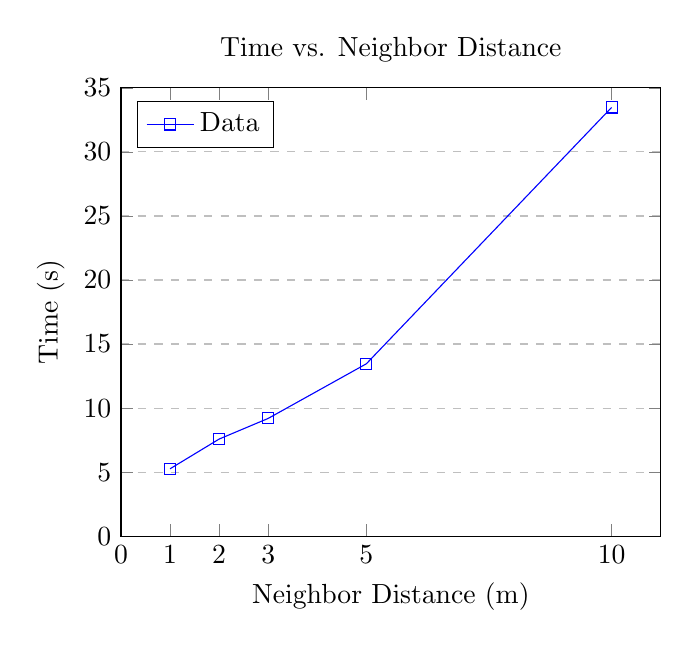
\begin{tikzpicture}
\begin{axis}[
    xlabel={Neighbor Distance (m)},
    ylabel={Time (s)},
    xmin=0, xmax=11,
    ymin=0, ymax=35,
    xtick={0,1,2,3,5,10},
    ytick={0,5,10,15,20,25,30,35},
    legend pos=north west,
    ymajorgrids=true,
    grid style=dashed,
    title={Time vs. Neighbor Distance},
]
\addplot[
    color=blue,
    mark=square,
    ]
    coordinates {
    (1, 5.262)(2, 7.583)(3, 9.195)(5, 13.457)(10, 33.472)
    };
    \legend{Data}
\end{axis}
\end{tikzpicture}
\caption{Graph Generation Time vs. Neighbor Distance (10,000 samples)}
\label{fig:time_distance}
\end{figure}

The two figures above give insight into the runtime for the graph generation, however the efficiency of the A* algorithm remains outstanding. While running the tests above, start and goal points on opposite sides of the map were selected to ensure functionality, and during all trials, the A* algorithm returned a path in less than 1 second. Due to this significant discrepancy in run time, it made sense only to consider the PRM generation in computational complexity as it is the rate-limiting step. The following evaluation was in the efficiency of the selected A* path. To quantitatively assess the efficiency, the following metrics were used: 

\begin{equation}
\text{path efficiency} = \frac{\text{actual path distance}}{\text{theoretical minimum path distance}}
\end{equation}

\begin{equation}
\text{path inefficiency} = \text{path efficiency} - 1
\end{equation}

The actual path distance was taken by summing the distances between the points returned in the A* algorithm, and the actual distance was calculated by finding the straight line distance between the start and the endpoint. To assess the algorithm under varying conditions, path efficiencies were calculated and are shown in the figure below:


\begin{figure}[H]
    \centering
    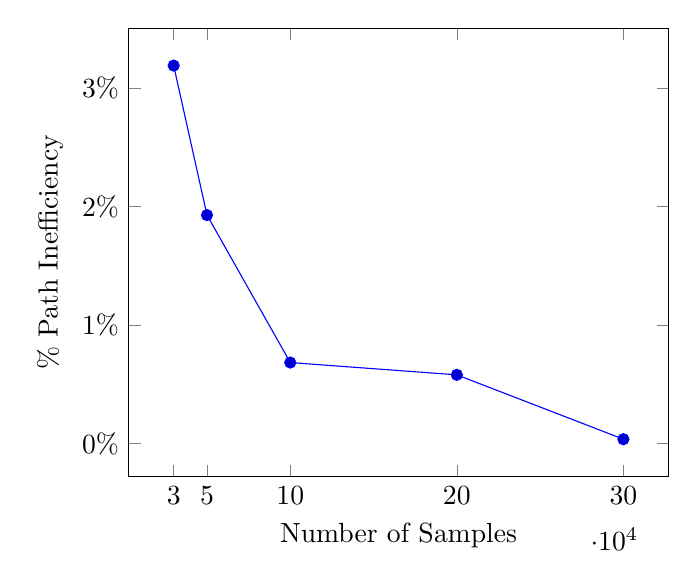
\begin{tikzpicture}
        \begin{axis}[
            xlabel={Number of Samples},
            ylabel={\% Path Inefficiency},
            xtick=data,
            xticklabels={ 3, 5, 10, 20, 30},
            yticklabel={\pgfmathprintnumber{\tick}\%},
            ]
            \addplot table {
               
                3000    3.188329013
                5000    1.927661855
                10000   0.6841701801
                20000   0.5804888129
                30000   0.0378350769
            };
        \end{axis}
    \end{tikzpicture}
    \caption{Path Efficiency vs. Number of Samples (50m run)}
    \label{fig:error_vs_samples}
\end{figure}

In this evaluation, a 50-meter-long stretch of track was used. Importantly, no path was returned when only 1,000 random samples were taken. From the data above, which certainly contains noise due to the random nature of the sampling, it appears that efficiency gains begin to diminish at 10,000 samples.

For further deployment in the same map, the optimal balance of computational and path efficiency appears to be 10,000 randomly generated samples with a "neighbor distance" of 5m. These parameters result in the generation of a graph and path in 15 seconds with an inefficiency of only $0.7\%$

\subsection{Pure Pursuit (Trajectory Follower): Thomas, Alex}
\subsubsection{Error in Line Follower}
To diagnose the error in our pure pursuit implementation, a graph was created to visualize the convergence of the distance to the line segment. At every callback, a variable named \texttt{dist2seg} was logged alongside the timestep it was recorded on. Then, this data was graphed using \texttt{matplotlib} and later evaluated to observe the algorithm's performance. We tested the robot on a sample, short-range start-to-end path consisting of four trajectory points along a right-bearing turn. The output graph is shown in Figure 7. 

Within the figure, large peaks are evident. The first peak is when the robot detects the trajectory's starting position, and drives straight towards it, decreasing distance error linearly. When it comes in contact with the line segment, it slowly converges to stability by calculating the appropriate steering angles. This is very stable on straight sections, and one can observe the robot quickly achieving a very low error term. 

Around the 75-second mark, another significant spike indicated that the robot has passed the halfway point of its current line segment and is now observing the starting node of the next line segment in the trajectory. It again travels linearly towards that point but then overshoots because this is the beginning of the right turn. It struggles to reduce the error at first because it can only turn in an arc while the line segment is linear, but once it completes the turn, it locks onto the segment and converges once again. 

This process repeats until it finds the endpoint of the trajectory and stops when a new goal point is given. From this process, we observed that our algorithm converges to the correct solution very efficiently, with a near-zero average error while within the bounds of the line segment, effectively ignoring the peaks before convergence. 

\begin{figure}[htbp]
  \centering
  \includegraphics[width=1\textwidth]{dist2seg_plot.png}
  \caption{Represents the distance error to the current line segment the robot is navigating towards.}
  \label{fig:failed_transform}
\end{figure}

\subsubsection{Adaptive Transformation}
After visualizing two different ways of transforming the look-ahead point from the map coordinate frame to the robot's coordinate frame, it was clear that the manual transformation using the robot's odometry to calculate the necessary rotation matrix was incorrect, and listening for the necessary transforms using RViz tools was the way to go. This situation arose because in this environment, the robot's information is its own pose and the position of the waypoints of the given trajectory. The waypoints are always in the map pursuit, and when testing pure pursuit in simulation without the particle filter, the robot's odometry is also broadcast in the map frame. Knowing this, the robot must be able to pursue the calculated target point, but since the algorithm was written assuming the target point is with respect to the robot's frame, it must be transformed into it. 

Let $p_r^m$ be the robot's position ($x$,$y$) with respect to the map, $p_t^m$ be the target point's position with respect to the map, and $R_r^m$ be the rotation matrix that transforms robot's position from its frame into the map frame. With this, the following relation exists:
\begin{equation}
    p_t^m = R_r^mp_t^r + p_r^m
\end{equation}
$p_t^r$ is the target point with respect to the robot's frame. Rearranging (3), the following relation exists:
\begin{equation}
    p_t^r = (R_r^m)^{-1}(p_t^m-p_r^m)
\end{equation}
Since we know the robot's pose with respect to the map frame, $\theta_r^m$ be the robot's orientation with respect to the map. With this, $(R_r^m)^{-1}=\begin{bmatrix}
    cos(\theta_r^m) & sin(\theta_r^m)\\
    -sin(\theta_r^m) & cos(\theta_r^m)\\
\end{bmatrix}$ and (4) can be written as:
\begin{equation}
    p_t^r = \begin{bmatrix}
    cos(\theta_r^m) & sin(\theta_r^m)\\
    -sin(\theta_r^m) & cos(\theta_r^m)\\
\end{bmatrix}(p_t^m-p_r^m)
\end{equation} and this retrieves the target point with respect to the robot frame, in theory. However, this was not the case, because after applying this relation to the given data, the transformed look-ahead point was visualized as shown below.

\begin{figure}[htbp]
  \centering
  \includegraphics[width=0.5\textwidth]{failed_transform.png}
  \caption{Transformed look-ahead point with respect to the robot. The point is ideally supposed to lie on the white line which represents the trajectory, but the calculation was incorrect, causing the point to lie at an undetermined offset position from the true look-ahead coordinates.}
  \label{fig:failed_transform}
\end{figure}

To fix this, ROS2 has a package called tf\_transformations which allows the robot to listen for transforms being published. This turned out to be the quickest, most effective solution. Using the lookup\_transform function, the robot to map transform was found, and after processing the \texttt{TransformStamped()} into a matrix representation of the pose, taking the inverse of it retrieved the transform of map to robot, $T_m^r$. Then, after constructing the corresponding matrix for the target point with respect to the map, $T_t^m$, simply matrix multiplying $T_m^r*T_t^m=T_t^r$   
To fix this, ROS2 has a package called \texttt{tf\_transformations} which allows the robot to listen for transforms being published. This turned out to be the quickest, most effective solution. Using the lookup\_transform function, the robot to map transform was found, and after processing the \texttt{TransformStamped()} into a matrix representation of the pose, taking the inverse of it retrieved the transform of map to robot, $T_m^r$. Then, after constructing the corresponding matrix for the target point with respect to the map, $T_t^m$, simply matrix multiplying $T_m^r*T_t^m$ yields $T_t^r$, the target point with respect to the robot. The successfully transformed look-ahead point is shown as the fuller purple arrow, the original look-ahead in the map frame as the red arrow, and the current segment as the two slender, purple arrows.
\begin{figure}[htbp]
  \centering
  \includegraphics[width=0.5\textwidth]{successful_transform.png}
  \caption{Transformed look-ahead point with respect to the robot. The point successfully lies on the white line which represents the trajectory and the untransformed point is in red.}
  \label{fig:failed_transform}
\end{figure}

\section{Conclusion: Alonso}

This lab culminated in the successful development and implementation of a probabilistic road map path planning algorithm within simulation as well as a pure pursuit controller to execute trajectories (TODO: in case we get it working on the robot). Each module works individually, as well as jointly, to randomly sample the space, create edges between nodes, return an optimal path using A*, and then execute odometry commands to follow said path.

Based upon our experimental evaluation, for path planning within the stata basement, the following set of conditions provided the best compromise between computational efficiency and path efficiency:

\begin{equation}
\text{number of samples} = 10,000
\end{equation}
\begin{equation}
\text{neighbor distance} = 5.0 m
\end{equation}

Moving forward, finalizing our integration of the algorithm on the robot is the next step. While this process has begun, there have been several difficulties between moving from simulation to the physical race car. Particularly for the final challenge, where path planning will be utilized in Luigi's mansion, ensuring accurate performance on the robot will be critical. 

As for work in simulation, other potential areas for improvement include further fine-tuning input parameters and making minor tweaks to improve runtime.


\section{Lessons Learned}

\subsection{Alonso}
I learned a lot about algorithm construction and communication best practices throughout this lab. I focused on the development of the path planning algorithm which was highly challenging. Through the development of the PRM algorithm, I found that writing a helper function to execute every step and then spending the time to figure out how to piece them together in the correct order was an efficient workflow. In past labs, I have attempted to write long blocks of code and found the debugging and logic much more difficult to complete. From a teamwork and communication perspective, this lab was a success. We were able to effectively plan and meet our internally set deadlines. Furthermore, we had the foresight to coordinate the syntax of the output of our path planner, which was the input of our trajectory follower. Due to the our effective communication and workflows, the integration on this lab was significantly easier than it was for the past lab. Moving forward to the final challenge, we will certainly implement the work practices we used for this lab.



\subsection{Heath}
While working on the path planning algorithm, I truly began to realize how important it was to have a general understanding of all the code contained within one project. For this lab in specific, there were many decisions about data structures and other elements of the included algorithms that, if not kept consistent, could lead to a major headache in the future. Seeings this potential problem, we did a fantastic job understanding which parts of our implementation to plan out before we began writing the code for this lab. This foresight made the integration part of this lab much easier, as the remaining tasks related to topic matching and visualization. Going forward I think it will be critical to meet as a group and all have an understanding for the components of our implementation to ensure that when tasks are being handled in parallel, each side is keeping their inputs and outputs consistent.

\subsection{Alex}
This lab reassured me of how important it is to ask for help and be open to working together on a problem with my teammates. As I worked on the pure pursuit code, there were a lot of small errors that if I tried to work on it by myself, it would have taken me a lot longer to find than working on it with Thomas and Marcelo, and asking for help from friends in the class or TAs. Additionally, we saw how effective proper communication between the two subteams fostered an environment that allowed for extremely easy integration, which includes adding good comments and docstrings to code and general updates either on discord on in person. This allowed us to make faster progress and allowed for easy integration.

\subsection{Thomas}
This lab has taught me a lot about the importance of working in parallel, task distribution, and communication throughout each step. I effectively commented and implemented doc-strings within my code so that my teammates could read, understand, and effectively add to it without needing in-person, lengthy explanations. It also minimized the risk of misinterpretation and causing rework later on in the process. I also experienced how important it was to diversify the topics in our teammates' code. Before this lab, I had little experience experimentally validating the performance of an algorithm I wrote in the form of plots. It was very challenging to figure out how to plot and interpret this data to effectively make changes to the program. This skill will be very useful going forward for our final project, where we will implement performance metrics along the way to make live updates to our code. 

\subsection{Marcelo}
With this lab, the main thing I learned was communication both in our code and in person. By designing our code to be interoperable and have consistent messages, we were able to avoid many of the pitfalls that come from having multiple modules being developed in parallel. Outside of our code, by communicating clearly, both in person and online, we were able to better plan and design our code. As such, we were able to make progress a lot faster than in some other labs.




\begin{thebibliography}{9}

\bibitem{MIT-RSS24}
MIT-RSS, ``Path Planning,'' GitHub, 2024. [Online]. Available: \url{https://github.com/mit-rss/path_planning}.

\vspace{0.5cm}

\bibitem{MIT-RSS24}
MIT-RSS, "Motion Planning 2 Lecture"

\bibitem{Stack Exchange}
Gareth Rees, "Line segment to circle collision algorithm", Stack Exhange, 2024 [Online]. Available: \url{https://codereview.stackexchange.com/questions/86421/line-segment-to-circle-collision-algorithm/86428#86428}

\end{thebibliography}


\end{document}